% DTT DIV in-vessel coil load model for disruption studies - Simscape implementation
% Rev. 00 - 2026-09-18 - compile with pdflatex (2 runs)
\documentclass[11pt,a4paper]{article}
\usepackage[margin=2.2cm]{geometry}
\usepackage[utf8]{inputenc}
\usepackage{amsmath,amssymb}
\usepackage{siunitx}
\sisetup{range-phrase=--, range-units=single, per-mode=symbol, detect-all}
\usepackage[european]{circuitikz}
\ctikzset{voltage dir=EF}  % voltage arrows from the higher to the lower potential (IEC 60375 / DIN 5489)
\usetikzlibrary{arrows.meta,positioning,calc}
\usepackage{graphicx}
\usepackage{booktabs}
\usepackage{array}
\newcolumntype{L}[1]{>{\raggedright\arraybackslash}p{#1}}
\usepackage{multirow}
\usepackage{caption}
\captionsetup{font=small,labelfont=bf}
\usepackage{fancyhdr}
\usepackage{xcolor}
\usepackage{enumitem}
\setlist{nosep}
\usepackage{listings}
\lstset{basicstyle=\ttfamily\footnotesize, breaklines=true, columns=fullflexible, frame=single, framerule=0.3pt, xleftmargin=4pt, keepspaces=true}
\usepackage[hidelinks,pdftitle={DTT DIV in-vessel coil load model for disruption studies - Rev. 00},pdfauthor={D. Bagnara}]{hyperref}
\usepackage[expansion=false]{microtype}

\newcommand{\docrev}{Rev.~00}
\newcommand{\docdate}{2026-09-18}
\newcommand{\doctitle}{DTT DIV in-vessel coil load model for disruption studies}
\newcommand{\code}[1]{\texttt{#1}}

\pagestyle{fancy}
\fancyhf{}
\lhead{\small \doctitle}
\rhead{\small \docrev\ -- \docdate}
\cfoot{\small Page \thepage}
\renewcommand{\headrulewidth}{0.4pt}

\title{\doctitle\\[4pt]\large Simscape (\code{.ssc}) implementation, identification on the ENEA specification curves and validation\\[6pt]\normalsize Technical note -- \docrev\ -- \docdate}
\author{D.~Bagnara}
\date{}

\begin{document}
\maketitle
\thispagestyle{fancy}

\begin{center}
\small
\begin{tabular}{@{}llp{9cm}@{}}
\toprule
\multicolumn{3}{@{}l}{\textbf{Revision history}}\\
\midrule
Rev. & Date & Description\\
\midrule
00 & 2026-09-18 & First issue. Load model of the DIV coils with the plasma-induced e.m.f., identified on Table~2, Fig.~3, Fig.~6 and Fig.~7 of ENEA specification PSS-SPT-59401 rev.~1.0; Simscape components \code{dtt.div\_coil}, \code{dtt.div\_coils3}, \code{dtt.emf\_table}, \code{dtt.emf\_analytic}, \code{dtt.plasma\_emf}; MATLAB parameter and validation scripts; digitised curves. Companion of the crowbar note \cite{crowbar_note} and of the $L_c$ reactor note \cite{lc_note}.\\
\bottomrule
\end{tabular}
\end{center}

\vspace{4pt}
\begin{abstract}
\noindent This note delivers a Simscape model of the DTT divertor in-vessel coils (DIV1, DIV2, DIV3) as seen from the power-supply terminals during a plasma disruption, so that the complete converter -- filter -- crowbar -- protection-coil circuit can be simulated in Simulink and the feasibility of the protection strategies can be documented. The coil is a Thevenin equivalent: the open-circuit e.m.f. $e(t)$ induced by the plasma (specification Fig.~6, digitised) in series with the coil resistance, self-inductance and two eddy-current loops identified on the frequency-dependent impedance of specification Fig.~3. The equations are exact for a linear system after the current quench and are implemented in Simscape language with the sign convention of the specification. The identification shows a fact that must be known before using the specification curves: the Fig.~7 crowbar current (\SI{10.9}{\kilo\ampere} peak, \SI{4.8}{\kilo\ampere} after \SI{300}{\milli\second}) is \emph{not} the response of the specified circuit to the Fig.~6 e.m.f., which gives only \SI{6.0}{\kilo\ampere}; it is reproduced within \SI{0.24}{\kilo\ampere} rms by the circuit of specification \S8.2 ($L_{coil}+L_{cab}+L_p = \SI{3.46}{\milli\henry}$, $R_{coil} = \SI{24.9}{\milli\ohm}$) driven by \num{1.84} times the Fig.~6 e.m.f. Both worst cases are therefore provided as parameter sets (\emph{voltage} worst case $k_e=1$, \emph{current} worst case $k_e=1.84$), together with a black-box R-L equivalent and a parametrised plasma-flux model (VDE growth, linear current quench, passive-structure delay) for what-if studies. The influence of the elements neglected by ENEA (cable and protection-coil resistance, eddy currents), of the quench duration and of the crowbar closing time is quantified, and the questions to be put to ENEA are listed.
\end{abstract}

\tableofcontents

\section{Scope and summary}
\label{sec:scope}
The crowbar note \cite{crowbar_note} established the duty of the DIV crowbar from the worst-case curves of the ENEA specification \cite{enea_spec} and the reactor note \cite{lc_note} designed the series reactor $L_c$ of the diode-bridge crowbar imposed by the customer. Both used a time-domain replica of the specification curves and simple R-L circuits. The next step, requested by the customer, is a load model usable inside a complete Simulink/Simscape model of the power supply (12-pulse rectifier, DC link, H-bridge, output filter, crowbar, protection coil), so that every situation -- disruption with the converter in current control, with the crowbar closed at different instants, with the fast dump active, with the converter in ``protection mode'', with the coils coupled -- can be tried and the limits of the decisions taken in the past can be documented with numbers.

The model is a Thevenin equivalent of the coil (Sec.~\ref{sec:model}): an e.m.f. $e(t)$ in series with the coil resistance $R_0$, the self-inductance $L_0$ and two eddy-current loops that represent the vacuum vessel and the passive structures. The e.m.f. is the open-circuit voltage induced by the plasma, i.e. specification Fig.~6, and the eddy loops are identified on the frequency-dependent inductance and resistance of specification Fig.~3. Five Simscape components are delivered (Sec.~\ref{sec:ssc}): the single coil, the three coupled coils, a table-driven e.m.f. source loaded with the digitised Fig.~6 curves, an analytic e.m.f. source parametrised by flux, growth rate, quench time and passive-structure delay, and an e.m.f. source driven by externally supplied plasma current and plasma--coil mutual inductance.

The identification (Sec.~\ref{sec:repro}) produced one result that changes how the specification curves must be read. Fig.~6 and Fig.~7 of \cite{enea_spec} are not consistent with each other through the circuit that the specification itself defines in \S8.2: with $L = L_{coil}+L_{cab}+L_p = \SI{3.46}{\milli\henry}$ and $R = R_{coil} = \SI{24.9}{\milli\ohm}$ (\S8.4 states that the cable and protection-coil resistances were not considered in Fig.~7) the Fig.~6 e.m.f. produces a crowbar current of \SI{6.0}{\kilo\ampere}, not \SI{10.9}{\kilo\ampere}. The Fig.~7 curve is reproduced within \SI{0.24}{\kilo\ampere} rms -- pre-quench dip, peak, time of the peak and tail -- by the same circuit driven by an e.m.f. \num{1.84} times larger than Fig.~6. Fig.~6 and Fig.~7 are therefore worst cases of two different quantities (voltage and current), presumably from two different disruption cases of the ENEA database, and a model that reproduces both needs a gain $k_e$ on the e.m.f.: $k_e = 1$ for the open-circuit voltage and the converter overvoltage, $k_e = 1.84$ for the crowbar current and $I^2t$. A single R-L black box (\SI{1.92}{\milli\henry}, \SI{13.1}{\milli\ohm}, \cite{crowbar_note}) reproduces Fig.~7 equally well but with an inductance and a resistance that have no physical meaning and that would falsify any simulation in which the converter is active; it is kept only as a cross-check.

The consequences for the protection studies are summarised in Sec.~\ref{sec:repro} and Sec.~\ref{sec:limits}: the induced current is imposed by the flux swing and not by the voltage peak (the peak current changes by less than 1\% when the quench duration is varied from \SI{1.5}{\milli\second} to \SI{12}{\milli\second}, while the voltage peak changes from \SI{6.5}{\kilo\volt} to \SI{2.5}{\kilo\volt}); 92\% of that flux reaches the coil through the passive structures with a \SI{26}{\milli\second} time constant, so the crowbar closing instant within a few milliseconds of the quench is irrelevant for the peak; the elements neglected by ENEA reduce the peak by \SIrange{3}{5}{\percent} and the $I^2t$ by \SIrange{16}{18}{\percent}; the protection coil halves the current that the crowbar would see without it. The main limits of the model are that the plasma response before the quench and the coil--coil mutual inductances are not available from the specification (Sec.~\ref{sec:limits}).

\section{Reference data}
\label{sec:data}
\subsection{Stand-alone parameters and frequency-dependent impedance}
Table~2 of \cite{enea_spec} gives the stand-alone coil parameters, the worst-case connection parameters (cables) and the protection-coil inductances (Table~\ref{tab:spec}). Fig.~3 of \cite{enea_spec} gives the equivalent inductance and resistance of the ``complete circuits'' (load coil plus protection coil, without connections) between \SI{0}{\hertz} and \SI{10}{\hertz}, computed by ENEA with the coupling to the passive structures. The inductance falls and the resistance rises with frequency (Fig.~\ref{fig:fig3}); the DC values (\SI{1.92}{}, \SI{1.68}{}, \SI{3.12}{\milli\henry}) are \SIrange{4}{7}{\percent} lower than the stand-alone sums (\SI{2.0}{}, \SI{1.8}{}, \SI{3.3}{\milli\henry}), which the specification attributes to ``coupling effects''. Note that the specification defines the Fig.~3 curves as ``the minimum achievable in the circuits'' and requires the Contractor to consider them.

\begin{table}[htbp]
\centering\small
\caption{Load data from \cite{enea_spec}, Table~2 and Fig.~3.}
\label{tab:spec}
\begin{tabular}{@{}lccc@{}}
\toprule
 & DIV1 & DIV2 & DIV3\\
\midrule
Stand-alone inductance $L_{coil}$ [mH] & 0.5 & 1.2 & 1.7\\
Stand-alone resistance $R_{coil}$ [m$\Omega$] & 10.6 & 18.7 & 24.9\\
Protection coil $L_p$ [mH] ($\pm$5\%) & 1.5 & 0.6 & 1.6\\
Connection (worst case, cables) & \multicolumn{3}{c}{\SI{160}{\micro\henry}, \SI{5}{\milli\ohm}}\\
Fig.~3 equivalent $L$ at DC / \SI{10}{\hertz} [mH] & 1.92 / 1.84 & 1.68 / 1.46 & 3.12 / 2.77\\
Fig.~3 equivalent $R$ at DC / \SI{10}{\hertz} [m$\Omega$] & 10.6 / 15.5 & 18.7 / 33.0 & 24.9 / 44.1\\
Open-circuit e.m.f. peak, Fig.~6 [kV] & $-5.9$ & $-5.9$ & $-2.9$\\
Crowbar current, Fig.~7 [kA] & -- & -- & 10.9 (+5 = 15.9)\\
\bottomrule
\end{tabular}
\end{table}

\begin{figure}[htbp]
\centering
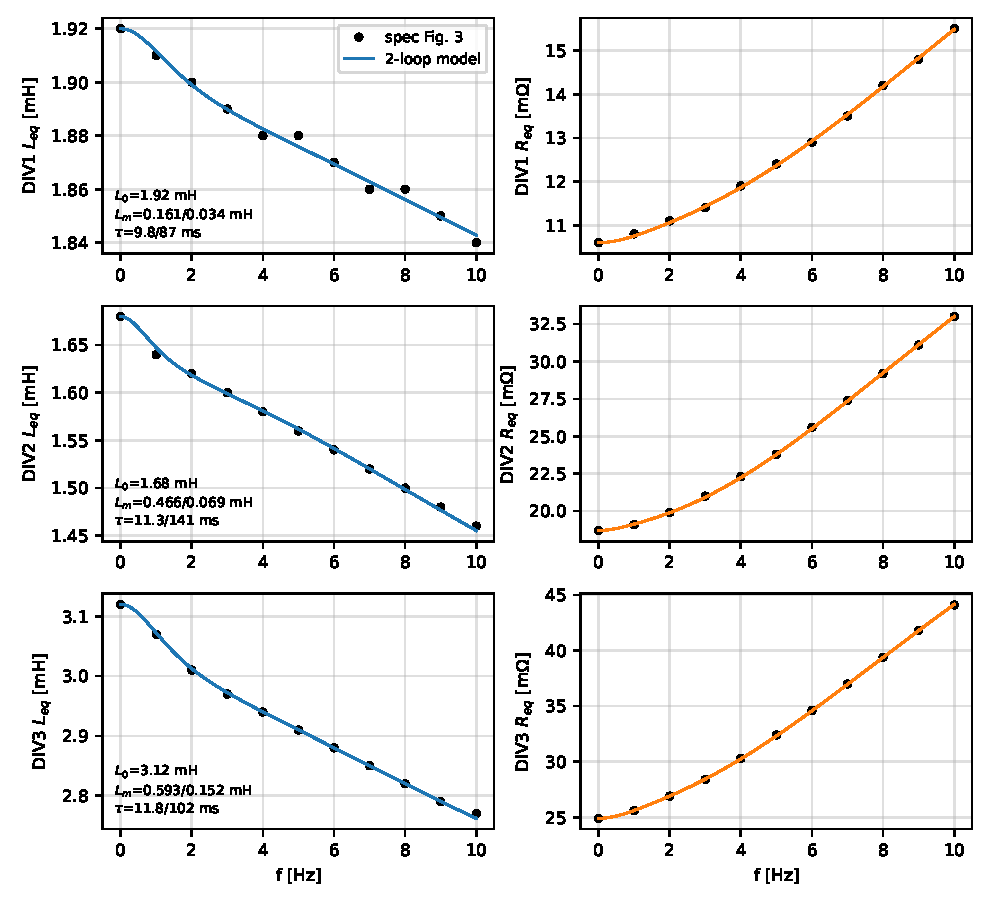
\includegraphics[width=0.9\textwidth]{fig/fig_fig3_fit}
\caption{Equivalent inductance and resistance of the three DIV circuits (coil + protection coil) from \cite{enea_spec} Fig.~3 (dots, values read from the figure labels) and the two-loop eddy-current model of Sec.~\ref{sec:eddy} (lines).}
\label{fig:fig3}
\end{figure}

\subsection{Disruption curves}
Fig.~6 of \cite{enea_spec} gives the voltage induced in the coils in the worst-case disruption with the coil circuit open; Fig.~7 gives, for DIV3 and an ideal crowbar, the induced overcurrent and its sum with the \SI{5}{\kilo\ampere} pre-disruption current. Both were digitised in \cite{crowbar_note} at \SI{0.05}{\milli\second} steps over \SIrange{0}{300}{\milli\second}; the curves are shown in Fig.~\ref{fig:emf} and are delivered as \code{data/dtt\_fig6\_fig7\_digitised.csv} after a light median filter that removes the grid-line artefacts of the digitisation without touching the quench spike (peak and flux preserved within 0.1\%). The accuracy is about 1\% of full scale.

The DIV3 e.m.f. has three phases: a slow positive growth to \SI{+344}{\volt} between \SI{0}{} and \SI{80}{\milli\second} (the plasma drifts towards the coil during the vertical displacement event, VDE), a negative spike to \SI{-2.86}{\kilo\volt} at \SI{83.3}{\milli\second} about \SI{3}{\milli\second} wide (the current quench), and a negative tail that decays with a time constant of about \SI{25}{\milli\second} (the currents induced in the vessel by the quench decay and their flux leaves the coil). The flux linked by the coil, $\int e\,dt$, is \SI{+7.2}{\weber} in the first phase, \SI{-36.8}{\weber} in the spike and tail, \SI{-29.6}{\weber} in total; for DIV1/DIV2 the total is \SI{-60.6}{\weber}. The tail carries most of the flux: only about 8\% of the quench flux reaches the coil during the \SI{3}{\milli\second} spike, the rest arrives through the passive structures over the following \SIrange{50}{100}{\milli\second}.

The Fig.~7 induced current starts negative (\SI{-3.2}{\kilo\ampere} at \SI{80}{\milli\second}, minimum \SI{-3.4}{\kilo\ampere}, in response to the positive pre-quench e.m.f.), crosses zero \SI{2}{\milli\second} after the spike, peaks at \SI{10.9}{\kilo\ampere} at \SI{139}{\milli\second}, i.e. \SI{56}{\milli\second} after the spike, and is \SI{4.8}{\kilo\ampere} at \SI{300}{\milli\second}. Its $I^2t$ over the \SI{300}{\milli\second} window is \SI{14.6}{\mega\ampere\squared\second} (\SI{38.1}{\mega\ampere\squared\second} for the total current with the constant \SI{5}{\kilo\ampere}, \SI{44}{\mega\ampere\squared\second} with the tail extrapolated to zero as done in \cite{crowbar_note}).

\begin{figure}[htbp]
\centering
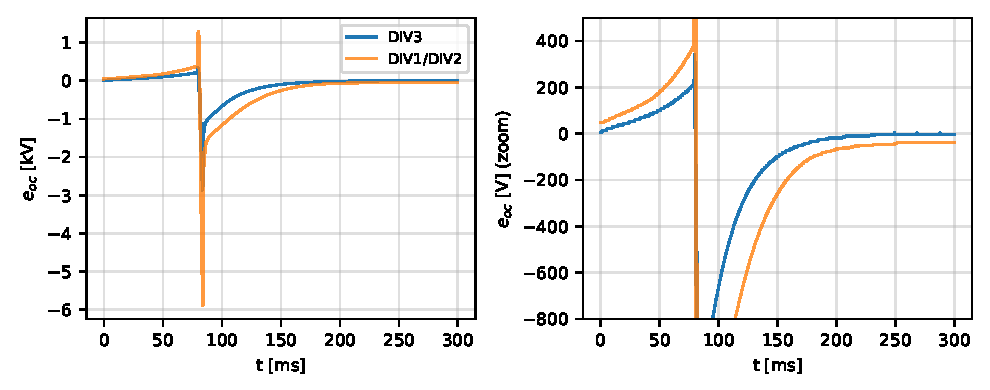
\includegraphics[width=0.95\textwidth]{fig/fig_emf_input}
\caption{Digitised open-circuit e.m.f. of \cite{enea_spec} Fig.~6 (ENEA sign convention): full scale (left) and zoom on the pre-quench growth and on the tail (right). These curves are the input \code{e} of the load model.}
\label{fig:emf}
\end{figure}

\subsection{Sign convention}
The specification plots the induced voltage positive during the VDE and negative at the quench, and the crowbar current positive. The model keeps exactly this convention: with the coil terminal $p$ connected to the positive output of the converter and the current $i$ counted into $p$, the terminal equation is $v = R_0 i + L_0\,di/dt + \dots + k_e\,e(t)$ with $e(t)$ the Fig.~6 curve as plotted. A short circuit ($v = 0$) then gives $i = -k_e e/(R + sL)$, i.e. the positive current of Fig.~7. The worst case of \S8.4 (pre-disruption current ``in the same direction of the induced overcurrent'') is $i_0 = +\SI{5}{\kilo\ampere}$; the opposite polarity of the disruption is obtained with $k_e < 0$, as \S8.5 requires the crowbar to be bidirectional because ``the curves in Figure~7 can occur in both directions''.

\section{Model equations}
\label{sec:model}
\subsection{Thevenin equivalent with eddy-current loops}
\label{sec:thevenin}
As long as the plasma current is an imposed source and the vessel, the passive structures and the other coils are linear, superposition applies to the coil terminals: the terminal voltage is the open-circuit response to the plasma (which contains the response of the passive structures to the plasma) plus the response to the coil current with the plasma removed,
\begin{equation}
v(s) = e_{oc}(s) + Z(s)\, i(s), \qquad Z(s) = R_0 + s L_0 - \sum_k \frac{s^2 M_k^2}{R_k + s L_k},
\label{eq:thevenin}
\end{equation}
where $Z(s)$ is the driving-point impedance of the coil coupled to $N$ passive loops ($L_k$, $R_k$, mutual $M_k$). This is exact after the current quench, when there is no plasma left and the system is passive; before the quench the plasma responds to the coil current (vertical instability) and Eq.~\eqref{eq:thevenin} neglects that response, which the specification does not provide either. Only the two combinations $L_{m,k} = M_k^2/L_k$ and $\tau_k = L_k/R_k$ enter $Z(s)$, so each loop is characterised by two numbers and can be referred to the coil by choosing $M_k = L_k = L_{m,k}$; its current $x_k$ then has the scale of the coil current. In the time domain (Fig.~\ref{fig:model})
\begin{align}
v &= R_0\, i + L_0\, \frac{di}{dt} + \sum_{k=1}^{N} L_{m,k}\, \frac{dx_k}{dt} + k_e\, e(t), \label{eq:coil}\\
0 &= \tau_k\, \frac{dx_k}{dt} + x_k + \tau_k\, \frac{di}{dt}, \qquad k = 1\dots N. \label{eq:loop}
\end{align}
The frequency-dependent inductance and resistance seen at the terminals are
\begin{equation}
L(\omega) = L_0 - \sum_k L_{m,k}\, \frac{(\omega\tau_k)^2}{1 + (\omega\tau_k)^2}, \qquad
R(\omega) = R_0 + \sum_k L_{m,k}\, \frac{\omega^2 \tau_k}{1 + (\omega\tau_k)^2},
\label{eq:LR}
\end{equation}
which is the form of the specification Fig.~3: $L$ drops from $L_0$ towards $L_0 - \sum_k L_{m,k}$ and $R$ rises from $R_0$, each loop contributing around $\omega \approx 1/\tau_k$. Eqs.~\eqref{eq:coil}--\eqref{eq:loop} are what the Simscape component \code{dtt.div\_coil} solves, with $N = 2$; the cable and the protection coil are left outside the component because they belong to the power supply and the user will want to vary them.

\begin{figure}[htbp]
\centering
% Equivalent circuit implemented in dtt.div_coil: R0, L0, e.m.f. e, two coupled eddy-current loops
\begin{circuitikz}[scale=1.0, every node/.style={font=\footnotesize}]
  \ctikzset{inductor=cute, inductors/scale=0.7, resistors/scale=0.8, sources/scale=0.7}
  % coil branch
  \draw (0,3) node[left]{$p$} to[short, o-, i=$i$] (0.8,3) to[R, l={$R_0$}] (2.4,3) to[L, l={$L_0$}, name=L0] (4.2,3) to[V, l={$k_e\,e(t)$}, name=E] (6.0,3) to[short, -o] (6.8,3) node[right]{$n$};
  \draw[-{Latex[length=2mm]}] (0.6,3.6) -- (6.2,3.6) node[midway, above] {$v = p.v - n.v$};
  % eddy loops
  \draw (2.4,1.4) to[L, l_={$L_1$}, name=L1] (4.2,1.4) to[R, l_={$R_1$}] (5.6,1.4) -- (5.6,0.6) -- (2.4,0.6) -- (2.4,1.4);
  \draw[-{Latex[length=1.6mm]}] (4.7,0.9) -- (3.5,0.9) node[midway, below] {$x_1$};
  \draw (2.4,-0.6) to[L, l_={$L_2$}, name=L2] (4.2,-0.6) to[R, l_={$R_2$}] (5.6,-0.6) -- (5.6,-1.4) -- (2.4,-1.4) -- (2.4,-0.6);
  \draw[-{Latex[length=1.6mm]}] (4.7,-1.1) -- (3.5,-1.1) node[midway, below] {$x_2$};
  % coupling marks
  \draw[<->, dashed, gray] (3.3,2.6) -- (3.3,1.8) node[midway, right] {$M_1$};
  \draw[<->, dashed, gray] (2.0,2.6) .. controls (1.4,1.2) .. (2.0,-0.2) node[pos=0.5, left] {$M_2$};
  \node[align=left, anchor=west] at (7.4,1.2) {passive structures\\(spec Fig.~3):\\$L_{m,k} = M_k^2/L_k$\\$\tau_k = L_k/R_k$\\ only $L_{m,k}$, $\tau_k$ matter};
  \node[align=left, anchor=west] at (7.4,-1.0) {$x_k$ = loop current\\referred to the coil ($M_k = L_k = L_{m,k}$)};
\end{circuitikz}

\caption{Equivalent circuit implemented in \code{dtt.div\_coil}: coil branch with the e.m.f. and two eddy-current loops coupled to it.}
\label{fig:model}
\end{figure}

\subsection{Identification of the eddy-current loops on Fig.~3}
\label{sec:eddy}
With $L_0$ and $R_0$ fixed at the DC values of Fig.~3, the loop parameters were fitted by least squares on the eleven labelled points of each curve (Table~\ref{tab:eddy}, Fig.~\ref{fig:fig3}). One loop is not enough (residual \SI{41}{\micro\henry} and \SI{0.66}{\milli\ohm} on DIV3); two loops reproduce all six curves within the resolution of the figure labels (\SI{3}{\micro\henry}, \SI{0.05}{\milli\ohm}); a third loop is not constrained by data limited to \SI{10}{\hertz}. The time constants are similar for the three coils (\SIrange{10}{12}{\milli\second} and \SIrange{90}{140}{\milli\second}), as expected for structures common to the three coils, and the coupling is strongest for DIV2 ($\sum L_m / L_0 = 32\%$) and DIV3 (24\%). The extrapolation of Eq.~\eqref{eq:LR} above \SI{10}{\hertz} is a hypothesis of the model: the high-frequency inductance $L_0 - \sum L_m$ (\SI{2.38}{\milli\henry} for the DIV3 circuit with $L_p$) is what the coil shows to the \SI{3}{\milli\second} quench spike, and faster loops that Fig.~3 cannot reveal would lower it further. Because 92\% of the disruption flux reaches the coil on the \SI{25}{\milli\second} time scale, this uncertainty has little effect on the crowbar current (Sec.~\ref{sec:variants}) but it matters for the voltage seen by the converter during the spike.

\begin{table}[htbp]
\centering\small
\caption{Two-loop eddy-current model of the three DIV circuits (coil + $L_p$) fitted on \cite{enea_spec} Fig.~3. The loops are attributed to the coil (the air-core protection coil has no frequency dependence); $L_0$ of the coil alone is $L_{dc} - L_p$ or the stand-alone value of Table~2.}
\label{tab:eddy}
\footnotesize
\begin{tabular}{@{}lcccccccc@{}}
\toprule
Circuit & $L_{dc}$ [mH] & $R_0$ [m$\Omega$] & $L_{m,1}$ [mH] & $\tau_1$ [ms] & $L_{m,2}$ [mH] & $\tau_2$ [ms] & $L_{dc}-\sum L_m$ [mH] & rms $L$ / $R$\\
\midrule
DIV1 & 1.92 & 10.6 & 0.161 & 9.8 & 0.034 & 86.9 & 1.73 & \SI{2}{\micro\henry} / \SI{0.03}{\milli\ohm}\\
DIV2 & 1.68 & 18.7 & 0.466 & 11.3 & 0.069 & 140.9 & 1.15 & \SI{3}{\micro\henry} / \SI{0.05}{\milli\ohm}\\
DIV3 & 3.12 & 24.9 & 0.593 & 11.8 & 0.152 & 102.3 & 2.38 & \SI{3}{\micro\henry} / \SI{0.04}{\milli\ohm}\\
\bottomrule
\end{tabular}
\end{table}

\subsection{Analytic plasma-flux model of the e.m.f.}
\label{sec:analytic}
For what-if studies (different quench durations, larger flux, disruption at a different instant, opposite polarity) a parametrised e.m.f. is more useful than a table. The physical picture of \cite{enea_spec} \S8.2 -- the coil links a flux $\Psi = M_{cp} I_p$ with the plasma -- is represented as follows. During the flat top the flux $\Psi_a = M_{cp,0} I_{p0}$ is constant and induces nothing; during the VDE the plasma approaches the coil, $M_{cp}$ grows and the flux increases by $\Delta\Psi_v$ with growth rate $g$; at $t_q$ the plasma current is quenched linearly to zero in $t_{cq}$; the vessel and the passive structures delay a fraction $\gamma$ of the flux variation with a time constant $\tau_v$:
\begin{align}
\Psi(t) &= \begin{cases} \Psi_a & t \le 0\\ \Psi_a + \Delta\Psi_v\, \dfrac{e^{g(t-t_q)} - e^{-g t_q}}{1 - e^{-g t_q}} & 0 < t \le t_q\\[6pt] (\Psi_a + \Delta\Psi_v)\left(1 - \dfrac{t - t_q}{t_{cq}}\right) & t_q < t < t_q + t_{cq}\\[4pt] 0 & t \ge t_q + t_{cq}\end{cases}\label{eq:psi}\\
e(t) &= (1-\gamma)\,\frac{d\Psi}{dt} + \gamma\, x, \qquad \tau_v \frac{dx}{dt} + x = \frac{d\Psi}{dt}. \label{eq:eanalytic}
\end{align}
The seven parameters were fitted on the digitised Fig.~6 (Table~\ref{tab:analytic}, Fig.~\ref{fig:analytic}). For DIV3 the fit reproduces the pre-quench growth, the tail and the total flux (\SI{-30.1}{} vs \SI{-29.6}{\weber}) within \SI{53}{\volt} rms; the single-time-constant delay smooths the spike (\SI{-2.30}{} vs \SI{-2.86}{\kilo\volt}), so for the converter overvoltage the digitised table is to be preferred, whereas for the crowbar current the analytic source gives the same result as the table within 2\% (\SI{11.28}{} vs \SI{11.05}{\kilo\ampere} in the circuit of Sec.~\ref{sec:repro}). The fitted values have a plausible physical reading: with $I_{p0} = \SI{5.5}{\mega\ampere}$ the plasma--coil mutual inductance is \SI{5.6}{\micro\henry} at flat top and \SI{7.7}{\micro\henry} at the quench for DIV3, the current quench lasts \SI{3.2}{\milli\second} ($dI_p/dt \approx \SI{1.7}{\giga\ampere\per\second}$, in the range of the ITPA database \cite{eidietis2015} for a machine of this size), and 92\% of the flux reaches the coil through the vessel with $\tau_v = \SI{26}{\milli\second}$, which is the order of magnitude of the DTT vacuum-vessel time constant. The DIV1/DIV2 fit is poorer (\SI{116}{\volt} rms) because their pre-quench curve has a sharp positive spike just before the quench (thermal quench) that Eq.~\eqref{eq:psi} does not describe.

\begin{table}[htbp]
\centering\small
\caption{Analytic e.m.f. model fitted on \cite{enea_spec} Fig.~6 (defaults of \code{dtt.emf\_analytic} and \code{par.plasma} in \code{dtt\_div\_params.m}).}
\label{tab:analytic}
\begin{tabular}{@{}lcccccccc@{}}
\toprule
Coil & $\Psi_a$ [Wb] & $\Delta\Psi_v$ [Wb] & $g$ [1/s] & $t_q$ [ms] & $t_{cq}$ [ms] & $\tau_v$ [ms] & $\gamma$ & rms [V]\\
\midrule
DIV3 & 30.6 & 11.9 & 31.8 & 81.1 & 3.19 & 25.8 & 0.92 & 53\\
DIV1/DIV2 & 62.9 & 24.7 & 1.3 & 81.6 & 2.70 & 37.6 & 0.91 & 116\\
\bottomrule
\end{tabular}
\end{table}

\begin{figure}[htbp]
\centering
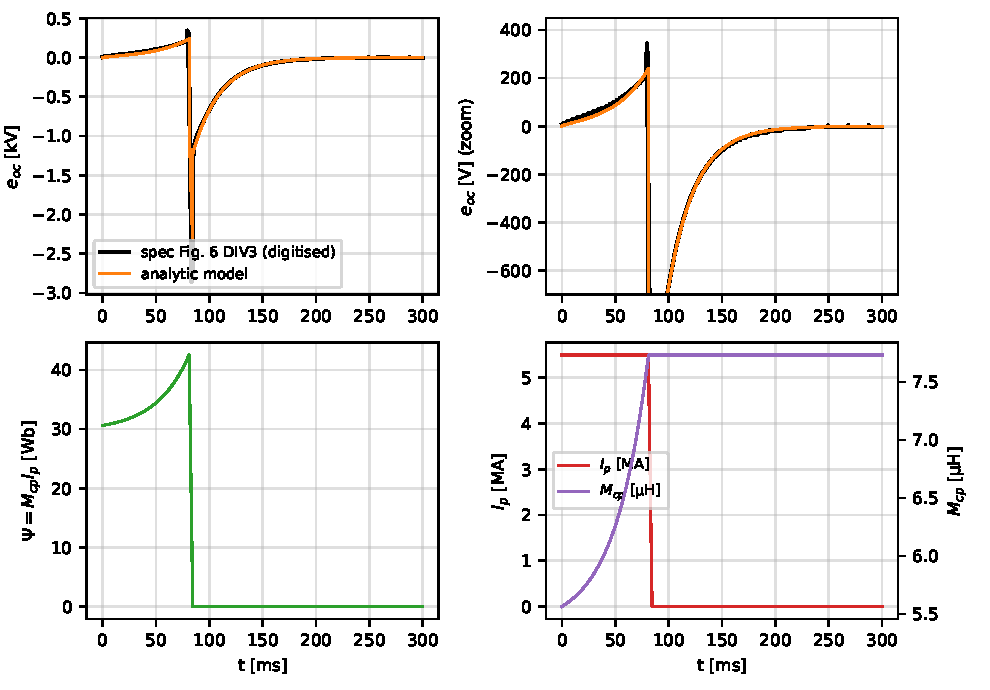
\includegraphics[width=0.95\textwidth]{fig/fig_analytic}
\caption{Analytic e.m.f. model (Eqs.~\eqref{eq:psi}--\eqref{eq:eanalytic}) against the digitised Fig.~6 for DIV3 (top), and the underlying flux, plasma current and mutual inductance trajectories (bottom) used by \code{dtt.emf\_analytic} and generated by \code{dtt\_plasma\_scenario.m} for \code{dtt.plasma\_emf}.}
\label{fig:analytic}
\end{figure}

\subsection{Three coupled coils}
\label{sec:coils3}
A disruption induces an e.m.f. in the three coils at the same time (Fig.~6), all three crowbars may close and the induced currents are coupled through the mutual inductances $M_{12}$, $M_{13}$, $M_{23}$ and through the common passive structures. The component \code{dtt.div\_coils3} implements
\begin{equation}
v_j = R_{0,j}\, i_j + \sum_{l=1}^{3} L_{jl}\, \frac{di_l}{dt} + \sum_{m=1}^{2} L_{m,jm}\, \frac{dx_{jm}}{dt} + k_{e,j}\, e_j(t), \qquad \tau_{jm}\, \frac{dx_{jm}}{dt} + x_{jm} + \tau_{jm}\, \frac{di_j}{dt} = 0,
\end{equation}
with the $3\times3$ inductance matrix $\mathbf{L}$ as a parameter. The specification does not give the mutual inductances (the default is $M = 0$, i.e. three independent coils); they must be requested from ENEA, together with the plasma-induced e.m.f. of the three coils for the same disruption case. An attempt to infer the mutuals from Fig.~7 alone (three coils shorted, Fig.~6 e.m.f.) was made and discarded: it requires negative mutuals of \SIrange{0.4}{0.7}{\milli\henry} and still misses the tail of Fig.~7, so the Fig.~7 current is not explained by coil--coil coupling.

\section{Reproduction of the specification curves}
\label{sec:repro}
\subsection{Fig.~6 does not produce Fig.~7 through the specified circuit}
\label{sec:fig7}
The specification states in \S8.2 that the overcurrent with an ideal crowbar is given by $v_{induced} \simeq (L_{coil}+L_{cable}+L_p)\,di/dt + (R_{coil}+R_{cable}+R_p)\,i$ and in \S8.4 that ``the actual overcurrent will be lower due to the effect of the resistance of the protection coil and of the connections (both not considered in the simulation in Figure~7)''. The circuit of Fig.~7 is therefore $L = \SI{1.7}{} + \SI{0.16}{} + \SI{1.6}{} = \SI{3.46}{\milli\henry}$ (or \SI{3.30}{\milli\henry} without the cable) and $R = \SI{24.9}{\milli\ohm}$, $\tau = L/R = \SI{139}{\milli\second}$. Driving this circuit with the digitised Fig.~6 DIV3 e.m.f. gives a peak of \SI{6.0}{\kilo\ampere} at \SI{139}{\milli\second} and \SI{2.35}{\kilo\ampere} at \SI{300}{\milli\second} (Fig.~\ref{fig:fig7}, green): the shape of Fig.~7 but 55\% of its amplitude. The eddy loops of Fig.~3 change this by less than 3\% (\SI{6.7}{\kilo\ampere}), a hypothetical fast loop tuned on the spike does not help because the flux arrives slowly, and a resistance free to vary reaches at most \SI{8.2}{\kilo\ampere} with \SI{7}{\milli\ohm} while spoiling the tail. In \cite{crowbar_note} Fig.~7 was reproduced with a free R-L fit, $L = \SI{1.92}{\milli\henry}$ and $R = \SI{13.1}{\milli\ohm}$ (rms \SI{0.21}{\kilo\ampere}); both values are \num{1.8}--\num{1.9} times smaller than those of the specified circuit while their ratio, the time constant, is the same (\SI{146}{} vs \SI{139}{\milli\second}).

This last observation gives the consistent explanation: since the circuit is linear, dividing $L$ and $R$ by the same factor is the same as multiplying the e.m.f. by that factor. Fitting a single gain $k_e$ on the Fig.~6 e.m.f. with the specified circuit gives $k_e = 1.84$ for \SI{3.46}{\milli\henry} (rms \SI{0.24}{\kilo\ampere}, peak \SI{11.05}{\kilo\ampere} at \SI{139}{\milli\second}, \SI{-3.23}{\kilo\ampere} at \SI{80}{\milli\second}, \SI{4.33}{\kilo\ampere} at \SI{300}{\milli\second}, $I^2t$ \SI{14.6}{\mega\ampere\squared\second} against \SI{14.6}{}) and $k_e = 1.79$ for \SI{3.30}{\milli\henry} (rms \SI{0.31}{\kilo\ampere}); leaving $R$ free as well returns $R = \SI{23.7}{\milli\ohm}$, i.e. the physical coil resistance. The whole curve is matched, including the pre-quench dip that depends only on the slow phase where no eddy effect can act (Fig.~\ref{fig:fig7}, left). The conclusion is that Fig.~7 was computed with the circuit of \S8.2 and with a disruption whose flux swing is \num{1.84} times that of Fig.~6 -- consistent with Fig.~6 being the worst case for the \emph{voltage} (fast quench) and Fig.~7 the worst case for the \emph{current} (largest flux swing, plasma closest to DIV3), taken from different cases of the ENEA disruption database. Whether the current-worst case also has a larger voltage peak cannot be known from the specification; with $k_e = 1.84$ applied to the Fig.~6 shape the model gives \SI{5.3}{\kilo\volt} open-circuit for DIV3, which is the conservative assumption for the converter until ENEA provides the e.m.f. of that case (Sec.~\ref{sec:limits}).

For the total current, Fig.~7 adds a constant \SI{5}{\kilo\ampere} to the induced current (the difference between the two ENEA curves is \SI{5.0}{\kilo\ampere} at every instant): the pre-disruption current is not let decay through the crowbar. In the model this corresponds to superposing \SI{5}{\kilo\ampere} to the result (peak \SI{16.05}{\kilo\ampere}, $I^2t$ \SI{37.9}{\mega\ampere\squared\second} over \SI{300}{\milli\second}, as ENEA); the physical alternative, $i_0 = \SI{5}{\kilo\ampere}$ decaying with the circuit time constant, gives \SI{12.9}{\kilo\ampere} and \SI{20.5}{\mega\ampere\squared\second} (Fig.~\ref{fig:fig7}, right). The ENEA superposition is the contractual one and is conservative.

\begin{figure}[htbp]
\centering
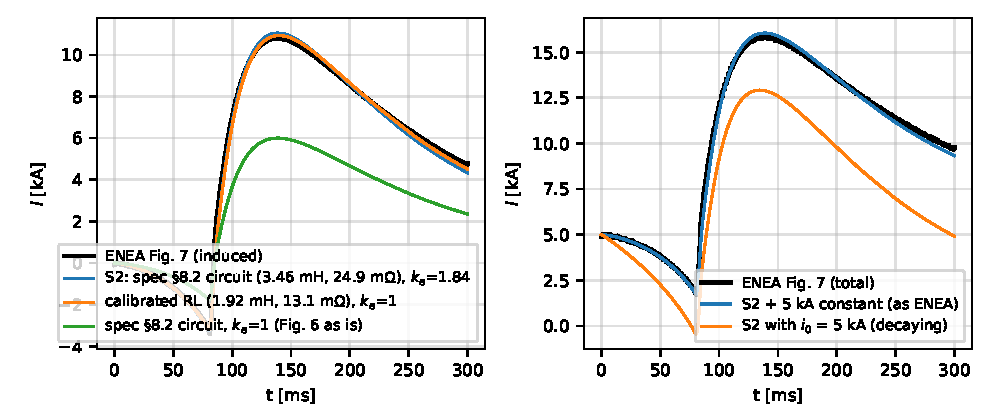
\includegraphics[width=0.95\textwidth]{fig/fig_fig7_repro}
\caption{Reproduction of \cite{enea_spec} Fig.~7 with an ideal crowbar. Left: induced current with the specified circuit (\SI{3.46}{\milli\henry}, \SI{24.9}{\milli\ohm}) and the Fig.~6 e.m.f. scaled by $k_e = 1.84$ (``S2'', orange), with the black-box R-L of \cite{crowbar_note} (blue) and with the specified circuit and the Fig.~6 e.m.f. as it is (green). Right: total current with the constant \SI{5}{\kilo\ampere} superposed as in the specification and with a decaying initial current.}
\label{fig:fig7}
\end{figure}

\subsection{Effect of the elements neglected in Fig.~7}
\label{sec:variants}
Starting from the ENEA-equivalent setting (S2) the elements that the specification declares neglected were added one at a time (Table~\ref{tab:variants}, Fig.~\ref{fig:variants}): the cable resistance (\SI{5}{\milli\ohm}, worst case of Table~2) and a placeholder \SI{1}{\milli\ohm} for the protection coil, the two eddy loops of Table~\ref{tab:eddy}, and the DC inductance of Fig.~3 instead of the stand-alone value. The resistances reduce the peak by 5\% and the $I^2t$ by 18\%, because they shorten the tail (\SI{3.2}{} instead of \SI{4.3}{\kilo\ampere} at \SI{300}{\milli\second}); the eddy loops raise the peak by 2\% (lower inductance on the \SI{25}{\milli\second} scale) and shorten the tail slightly; the lower DC inductance of Fig.~3 raises the peak by 4\%. The spread between the variants is within the accuracy of the reference curves, so the S2 setting is an adequate and conservative representation of the current worst case for the crowbar, while the variants bracket the real circuit. The last row shows why the protection coil exists: without $L_p$ the peak is \SI{16.8}{\kilo\ampere} (\SI{21.8}{\kilo\ampere} with the \SI{5}{\kilo\ampere}) and the $I^2t$ is 52\% higher. The right panel of Fig.~\ref{fig:variants} gives the sensitivity to the e.m.f. gain for the fully physical set: the current scales linearly with $k_e$, from \SI{5.9}{\kilo\ampere} at $k_e = 1$ to \SI{12.9}{\kilo\ampere} at $k_e = 2.2$.

\begin{table}[htbp]
\centering\small
\caption{Ideal-crowbar current of DIV3 with the Fig.~6 e.m.f. scaled by $k_e = 1.84$, for the ENEA-equivalent circuit and its physical variants. $I^2t$ over \SIrange{0}{300}{\milli\second}; ``total'' = induced + \SI{5}{\kilo\ampere} constant.}
\label{tab:variants}
\footnotesize
\begin{tabular}{@{}lccccc@{}}
\toprule
Circuit & Peak [kA] & at [ms] & $i$(\SI{300}{\milli\second}) [kA] & $I^2t$ [MA$^2$s] & $I^2t$ total [MA$^2$s]\\
\midrule
ENEA Fig.~7 (digitised) & 10.9 & 139 & 4.79 & 14.6 & 38.1\\
S2: \SI{3.46}{\milli\henry}, $R = R_{coil}$ & 11.05 & 139 & 4.33 & 14.6 & 37.9\\
+ $R_{cab}$ \SI{5}{\milli\ohm} + $R_p$ \SI{1}{\milli\ohm} & 10.53 & 134 & 3.19 & 12.0 & 33.5\\
+ eddy loops (Fig.~3) & 10.77 & 129 & 3.05 & 12.2 & 33.7\\
+ eddy loops, $L_0 = L_{dc} - L_p = \SI{1.52}{\milli\henry}$ & 11.24 & 128 & 2.94 & 12.9 & 34.7\\
Without $L_p$ (coil + cable, $R_{coil}+R_{cab}$) & 16.77 & 123 & 1.74 & 22.1 & 46.8\\
\bottomrule
\end{tabular}
\end{table}

\begin{figure}[htbp]
\centering
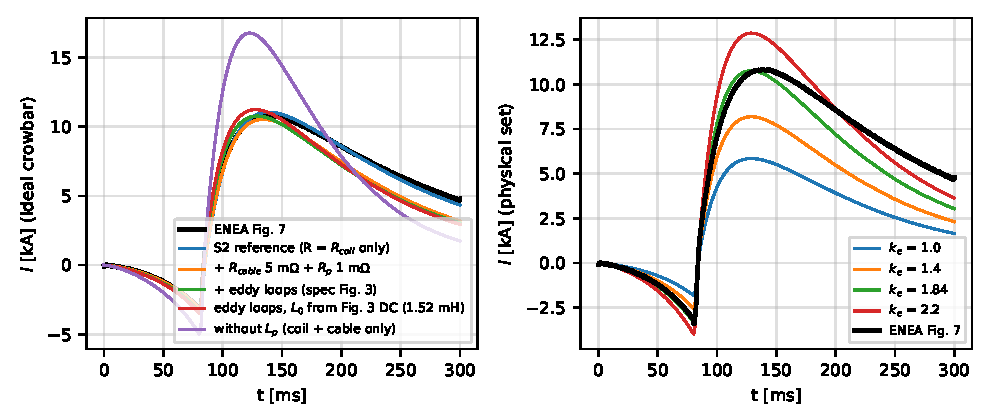
\includegraphics[width=0.95\textwidth]{fig/fig_physical_variants}
\caption{Left: the physical variants of Table~\ref{tab:variants}. Right: sensitivity of the fully physical set (resistances and eddy loops included) to the e.m.f. gain $k_e$.}
\label{fig:variants}
\end{figure}

\subsection{Quench duration and crowbar closing time}
\label{sec:whatif}
Two what-if cases with the analytic e.m.f. illustrate the ``current generator'' behaviour of the load (Fig.~\ref{fig:whatif}). Varying the current-quench duration from \SI{1.5}{} to \SI{12}{\milli\second} at constant flux changes the peak voltage from \SI{-6.5}{} to \SI{-2.5}{\kilo\volt} ($k_e = 1.84$, DIV3) but the peak crowbar current only from \SI{11.15}{} to \SI{11.23}{\kilo\ampere}: the current is set by the flux swing, by the circuit inductance and by the ratio between the delivery time and the circuit time constant, not by the voltage. The converter sees the voltage; the crowbar sees the flux.

The second case delays the closing of an otherwise open circuit (the coil carries no current until the crowbar closes -- an idealisation, since the converter freewheeling diodes would conduct). Closing at \SI{85}{\milli\second}, \SI{2}{\milli\second} after the spike, gives the same peak as closing at $t = 0$ (\SI{10.99}{} vs \SI{11.05}{\kilo\ampere}), because 92\% of the flux is still to come through the vessel; closing at \SI{100}{\milli\second} gives \SI{6.2}{\kilo\ampere}, at \SI{130}{\milli\second} \SI{2.0}{\kilo\ampere}. Two consequences for the protection strategy: the crowbar trigger delay (tens of microseconds, \cite{crowbar_note}) is irrelevant for the current duty, and whatever absorbs flux before the crowbar closes reduces the crowbar current one-to-one. An H-bridge in protection mode applying \SI{600}{\volt} against the e.m.f. absorbs about \SI{30}{\weber} in \SI{50}{\milli\second}, i.e. roughly half of the \SI{68}{\weber} of the current worst case, but it must return the corresponding energy (of the order of \SI{300}{\kilo\joule}) to the DC link, which the \SI{665}{\milli\farad} bank cannot take without the fast dump; this is precisely the kind of trade-off the complete Simscape model is meant to quantify.

\begin{figure}[htbp]
\centering
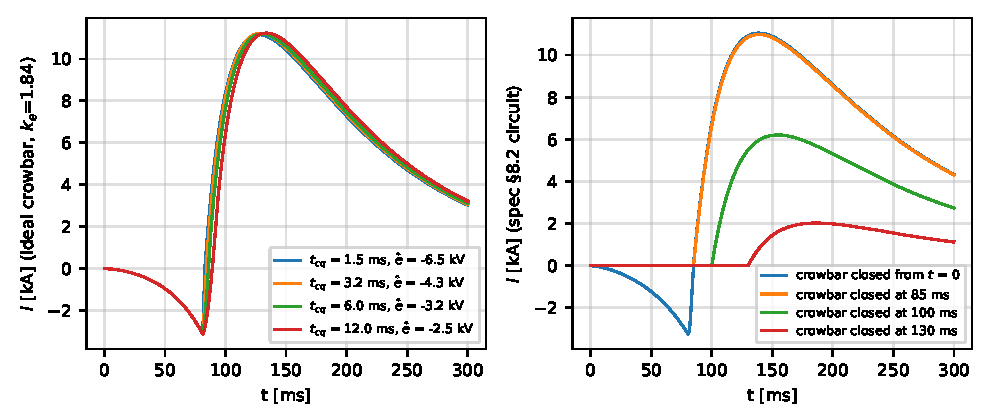
\includegraphics[width=0.95\textwidth]{fig/fig_whatif}
\caption{Left: ideal-crowbar current for different current-quench durations at constant flux (analytic e.m.f., $k_e = 1.84$, physical set); the legend gives the corresponding e.m.f. peak. Right: effect of the crowbar closing instant with the coil open until then (S2 setting).}
\label{fig:whatif}
\end{figure}

\section{Simscape implementation}
\label{sec:ssc}
\subsection{Components}
The package \code{ssc/+dtt} contains five components in Simscape language (Table~\ref{tab:blocks}); \code{ssc\_build dtt} run in the \code{ssc} folder generates the library \code{dtt\_lib}. All electrical ports are Foundation-library electrical conserving ports; the e.m.f. and the plasma quantities are physical signals so that they can come from Simulink (From Workspace, Signal Builder, a lookup table or a plasma model) through a Simulink--PS converter, or directly from the delivered sources.

\begin{table}[htbp]
\centering\small
\caption{Simscape components delivered (package \code{dtt}, library \code{dtt\_lib}).}
\label{tab:blocks}
\begin{tabular}{@{}L{3.2cm}L{4.2cm}L{8.2cm}@{}}
\toprule
Block (file) & Ports & Parameters (defaults)\\
\midrule
DIV Coil (\code{div\_coil.ssc}) & $p$, $n$ electrical; \code{e} PS input [V]; \code{i} PS output [A] & $R_0$ \SI{24.9}{\milli\ohm}, $L_0$ \SI{1.7}{\milli\henry}, $L_{m1}$ \SI{0.593}{\milli\henry}, $\tau_1$ \SI{11.8}{\milli\second}, $L_{m2}$ \SI{0.152}{\milli\henry}, $\tau_2$ \SI{102}{\milli\second}, $k_e$ 1, $i_0$ 0 (DIV3 values; set $L_{m1} = L_{m2} = 0$ for a pure R-L)\\
DIV Coils 3 (\code{div\_coils3.ssc}) & $p_j$, $n_j$ ($j = 1,2,3$); \code{e1..e3} PS inputs & $\mathbf{R}_0$ [10.6 18.7 24.9] m$\Omega$, $\mathbf{L}$ diag(0.5, 1.2, 1.7) mH with $M = 0$, $\mathbf{L}_m$, $\boldsymbol{\tau}$ ($3\times2$, Table~\ref{tab:eddy}), $\mathbf{k}_e$, $i_{10}$, $i_{20}$, $i_{30}$\\
EMF Table (\code{emf\_table.ssc}) & \code{e} PS output & \code{t\_tab}, \code{e\_tab} (vectors, e.g. \code{C.t}, \code{C.e\_div3}), $t_0$, $k$; linear interpolation, end values held\\
EMF Analytic (\code{emf\_analytic.ssc}) & \code{e}, \code{Psi} PS outputs & $\Psi_a$, $\Delta\Psi_v$, $g$, $t_q$, $t_{cq}$, $\tau_v$, $\gamma$ (Table~\ref{tab:analytic}, DIV3), $t_0$, $k$\\
Plasma EMF (\code{plasma\_emf.ssc}) & \code{Ip} [A], \code{Mcp} [H] PS inputs; \code{e}, \code{Psi} PS outputs & $\tau_v$, $\gamma$, derivative filter $\tau_f$ \SI{50}{\micro\second}, $k$, $\Psi_{init}$ (initial $M_{cp} I_p$)\\
\bottomrule
\end{tabular}
\end{table}

The coil component declares the currents $i$, $x_1$, $x_2$ as high-priority initial conditions ($i_0$, 0, 0), which is consistent with a DC pre-disruption current; the eddy-loop equations contain $di/dt$ and the coil equation $dx_k/dt$, an index-1 system that Simscape handles like coupled inductors. The Plasma EMF block obtains the flux derivative with a first-order filter ($\tau_f \ll t_{cq}$) and initialises the filter states at $\Psi_{init}$ to avoid a start-up spike; alternatively the ``Start simulation from steady state'' option of the Solver Configuration block can be used. The analytic source uses the simulation time in conditional equations (\code{if time - t0 <= tq \dots}), which is legal in Simscape language; the piecewise definition creates zero crossings at $t_0$, $t_0 + t_q$ and $t_0 + t_q + t_{cq}$.

\subsection{Connection and conventions}
Fig.~\ref{fig:usage} shows where the block sits: the cable and the protection coil are external series elements between the crowbar node and the coil; the filter capacitor of the power supply is across the converter side. The sign convention is that of Sec.~\ref{sec:data}: $p$ to the positive converter terminal, $e$ as plotted in the specification, $i_0 = +\SI{5}{\kilo\ampere}$ for the worst case, $k_e < 0$ for the opposite polarity. The block is inductive at its terminals, so it can be connected to any node of the converter model, including a capacitor node, without topological conflicts; a current sensor or the PS output \code{i} gives the coil current. When a pre-disruption current $i_0 \neq 0$ is set in the block, the same initial current must be given to the external series inductors (cable, $L_p$), otherwise Simscape reports conflicting high-priority initial targets.

\begin{figure}[htbp]
\centering
% How the load model sits in the DIV3 circuit (validation circuit = crowbar closed, converter removed)
\begin{circuitikz}[scale=0.86, transform shape, every node/.style={font=\footnotesize}]
  \ctikzset{inductor=cute, inductors/scale=0.7, capacitors/scale=0.8, resistors/scale=0.8, sources/scale=0.7}
  % converter box
  \draw (0,0) rectangle (2.2,3.4); \node[align=center] at (1.1,1.7) {H-bridge\\$\pm$\SI{600}{\volt}\\$\pm$\SI{5}{\kilo\ampere}\\+ output\\filter};
  \draw (2.2,3.0) -- (3.6,3.0); \draw (2.2,0.4) -- (3.6,0.4);
  % crowbar
  \draw (3.6,3.0) -- (3.6,2.5) to[Ty, invert] (3.6,0.9) -- (3.6,0.4);
  \node[anchor=west] at (3.8,1.7) {crowbar};
  % series elements
  \draw (3.6,3.0) -- (4.8,3.0) to[L, l={$L_p$ \SI{1.6}{\milli\henry}}] (6.3,3.0) to[R, l_={$R_p$}] (7.5,3.0) to[L, l={$L_{cab}$ \SI{160}{\micro\henry}}] (9.0,3.0) to[R, l_={$R_{cab}$ \SI{5}{\milli\ohm}}] (10.2,3.0) to[short, i=$i$] (11.2,3.0);
  \draw (3.6,0.4) -- (11.2,0.4);
  % DIV coil block
  \draw[thick] (11.2,-0.5) rectangle (15.8,3.9);
  \node[anchor=south west] at (11.2,3.95) {\textbf{DIV Coil} (\texttt{dtt.div\_coil})};
  \draw (11.2,3.0) node[above left=1pt and 0pt]{$p$} -- (11.6,3.0) to[R, l={$R_0$}] (12.7,3.0) to[L, l={$L_0$}] (13.8,3.0) -- (14.6,3.0) to[V, l={$k_e e$}] (14.6,1.4) -- (14.6,0.4) -- (11.2,0.4) node[below left=1pt and 0pt]{$n$};
  \draw (11.8,1.9) to[L, l_={$L_1$}] (12.8,1.9) to[R, l_={$R_1$}] (13.8,1.9) -- (13.8,1.2) -- (11.8,1.2) -- (11.8,1.9);
  \draw[<->, dashed, gray] (12.3,2.7) -- (12.3,2.1);
  \node[anchor=north] at (13.3,0.95) {eddy loops (spec Fig.~3)};
  % emf source
  \draw[thick] (16.8,1.2) rectangle (19.2,2.4); \node[align=center] at (18.0,1.8) {EMF Table /\\EMF Analytic};
  \draw[-{Latex[length=2mm]}] (16.8,1.8) -- (15.8,1.8) node[midway, above] {$e$};
  % voltage arrow
  \draw[-{Latex[length=2mm]}] (10.8,2.8) -- (10.8,0.6) node[midway, left] {$v$};
  % note
  \node[align=left, anchor=north west, text width=10.5cm] at (3.6,-0.7) {Sign convention: $i$ into $p$; $v = R_0 i + L_0\,di/dt + L_{m1}\,dx_1/dt + L_{m2}\,dx_2/dt + k_e e$. An ideal crowbar ($v = 0$) with $e$ = spec Fig.~6 (negative spike) gives the positive induced current of spec Fig.~7; worst case with $i_0 = +\SI{5}{\kilo\ampere}$; opposite polarity with $k_e < 0$.};
\end{circuitikz}

\caption{Position of the load model in the DIV3 circuit and sign convention. The validation circuit of Sec.~\ref{sec:valid} is this one with the crowbar closed and the converter removed.}
\label{fig:usage}
\end{figure}

\subsection{Parameter sets}
\label{sec:params}
The function \code{dtt\_div\_params.m} returns all the parameter sets of Table~\ref{tab:sets}. The recommended use is: physical set for everything that involves the converter (control, normal operation, overvoltage, protection mode), with the e.m.f. table at $k_e = 1$ for the voltage worst case and at $k_e = 1.84$ for the current worst case; ENEA-equivalent set when the purpose is to reproduce the contractual Fig.~7 (e.g. crowbar $I^2t$ verification in the FDR); black-box set only as a cross-check.

\begin{table}[htbp]
\centering\small
\caption{Parameter sets for DIV3 (\code{dtt\_div\_params.m}). Cable and $L_p$ are always external.}
\label{tab:sets}
\begin{tabular}{@{}L{3.4cm}L{6.4cm}L{5.6cm}@{}}
\toprule
Set & DIV Coil block & External / e.m.f.\\
\midrule
Physical (\code{par.div3}) & $R_0$ \SI{24.9}{\milli\ohm}, $L_0$ \SI{1.7}{\milli\henry} (or \SI{1.52}{\milli\henry} = Fig.~3 DC $- L_p$), eddy loops of Table~\ref{tab:eddy} & cable \SI{160}{\micro\henry}/\SI{5}{\milli\ohm}, $L_p$ \SI{1.6}{\milli\henry} with its real $R_p$; \code{e} = Fig.~6 table, $k = 1$ (voltage) or 1.84 (current)\\
ENEA-equivalent (\code{par.enea}) & $R_0$ \SI{24.9}{\milli\ohm}, $L_0$ \SI{1.7}{\milli\henry}, $L_{m} = 0$ & cable \SI{160}{\micro\henry}/\SI{0}{}, $L_p$ \SI{1.6}{\milli\henry}/\SI{0}{}; \code{e} = Fig.~6 table, $k = 1.84$; reproduces Fig.~7 (rms \SI{0.24}{\kilo\ampere}); total = + \SI{5}{\kilo\ampere}\\
Black box (\code{par.calib}) & $R_0$ \SI{13.1}{\milli\ohm}, $L_0$ \SI{1.92}{\milli\henry}, $L_m = 0$, whole loop lumped & no cable, no $L_p$; \code{e} = Fig.~6 table, $k = 1$; cross-check only\\
Analytic plasma (\code{par.plasma}) & physical set & EMF Analytic or Plasma EMF with Table~\ref{tab:analytic}; scale $k$, vary $t_{cq}$, $\Delta\Psi_v$, $t_0$\\
\bottomrule
\end{tabular}
\end{table}

\subsection{Validation procedure}
\label{sec:valid}
No MATLAB installation was available where this note was written, so the components were written against the Simscape language specification \cite{simscape_lang} and verified with a Python replica of Eqs.~\eqref{eq:coil}--\eqref{eq:loop} (exact discretisation of the linear state-space model, \code{py/divmodel.py}); all figures and numbers of this note come from that replica. Two MATLAB scripts allow the user to close the loop:
\begin{enumerate}[label=(\arabic*)]
\item \code{dtt\_validate\_ode.m} (no Simulink needed): loads the CSV, runs the same equations with a trapezoidal integrator (\code{dtt\_sim\_coil.m}) and must give the numbers of Table~\ref{tab:variants} first three rows and of Table~\ref{tab:analytic}; this checks the data files and the parameter sets.
\item \code{dtt\_build\_validation\_model.m}: after running \code{ssc\_build dtt} it builds, programmatically, the Simulink model of Fig.~\ref{fig:usage} (named \code{dtt\_div\_validation}) with the crowbar closed (EMF Table, DIV Coil, $L_{cab}$, $L_p$ and a current sensor in one closed loop), runs it with \code{ode23t} and overlays the result on Fig.~7; expected: peak \SI{11.05}{\kilo\ampere} at \SI{139}{\milli\second}, \SI{4.33}{\kilo\ampere} at \SI{300}{\milli\second}. The automatic wiring relies on the port numbering of the generated blocks (physical-signal ports first, as in the Foundation library: left \code{e}, $p$; right \code{i}, $n$); if it fails the blocks are left in place for manual wiring.
\end{enumerate}
Solver hints: the quench spike has a \SI{3}{\milli\second} width and the tail \SI{25}{\milli\second}, so a maximum step of \SI{50}{\micro\second} is adequate for the load alone; in the complete model the converter switching (\SI{4}{\kilo\hertz}, \SI{200}{\nano\second} jitter) dictates the step. \code{ode23t} or \code{ode15s} with relative tolerance \num{1e-5}; with the table source the interpolation is linear, so a variable-step solver will not miss the spike.

\subsection{Scenarios to explore with the complete model}
\label{sec:scenarios}
The following list is the proposed test matrix for the complete power-supply model, in the order in which the results build on each other:
\begin{enumerate}[label=S\arabic*.]
\item Ideal crowbar closed from $t = 0$, ENEA-equivalent set: reproduces Fig.~7 (regression test of the model).
\item Converter in current control at $\pm\SI{5}{\kilo\ampere}$ and at zero, no crowbar action, $k_e = 1$ and $1.84$, both polarities: terminal voltage, current excursion, DC-link voltage, IGBT current -- this defines the overvoltage and the current the converter must survive until the crowbar closes and quantifies \S8.4 ``the induced voltage is high, but it is not totally seen by the PS''.
\item Crowbar (real model: diode bridge, thyristor, $L_c$ \cite{lc_note}, BOD level) triggered by the terminal voltage or current thresholds: firing instant, thyristor peak, $I^2t$, energy; then with the firing delayed by \SI{1}{}, \SI{2}{}, \SI{5}{}, \SI{10}{}, \SI{20}{\milli\second} (the \SI{25}{\milli\second} flux delivery makes the duty insensitive to small delays, Sec.~\ref{sec:whatif}).
\item Protection mode of the converter (drive the current to zero with $\pm\SI{600}{\volt}$) with and without the crowbar, with the fast dump enabled: flux absorbed, DC-link excursion, dump energy -- the feasibility limit of managing the disruption without crowbar (\S8.4 last paragraph).
\item Quench duration \SIrange{1.5}{12}{\milli\second}, flux $\pm 30\%$ (analytic source): margins on the voltage-based trigger and on the thyristor rating.
\item Three coils with \code{DIV Coils 3}, all crowbars closing, $M = 0$ and then the ENEA matrix when available; DIV1/DIV2 with their own e.m.f. (\SI{-5.9}{\kilo\volt}, \SI{-60.6}{\weber}): the current-worst case of the other two crowbars, which the specification does not give.
\item Disruption during a \SI{10}{\hertz} full-current waveform (the coil current is not DC when the disruption comes): initial conditions of the eddy loops and of the filter.
\end{enumerate}

\section{Limits and open points}
\label{sec:limits}
\begin{itemize}[leftmargin=*]
\item \textbf{Fig.~6 and Fig.~7 are different cases.} The gain $k_e = 1.84$ is inferred, not given. ENEA should be asked for the open-circuit e.m.f. of the three coils in the disruption case used for Fig.~7 (and its voltage peak), and to confirm the circuit parameters used for Fig.~7 (coil + cable + $L_p$, $R_{coil}$ only). Until then the model uses the Fig.~6 shape at $k_e = 1.84$ for the current and, conservatively, also for the voltage (\SI{5.3}{\kilo\volt} open circuit).
\item \textbf{Plasma response before the quench.} During the VDE the plasma responds to the coil current; the Thevenin model ignores it (Eq.~\eqref{eq:thevenin} is exact only after the quench). The effect is confined to the \SI{80}{\milli\second} of small e.m.f. and to the initial dip of the current, and the fit of the pre-quench dip of Fig.~7 suggests it is small for the shorted circuit; it may matter for the converter in current control, where the coil field acts on the plasma position. ENEA's ``more detailed models'' (\S4.2) would be the plasma-response linear model (CREATE-L type), which can be inserted as a Simulink block feeding \code{Plasma EMF}.
\item \textbf{Eddy loops above \SI{10}{\hertz}.} The extrapolation of Table~\ref{tab:eddy} beyond \SI{10}{\hertz} is a hypothesis; it affects the voltage division during the \SI{3}{\milli\second} spike and the ripple current at \SI{4}{\kilo\hertz} (the passive structures reduce the inductance seen by the switching frequency), not the crowbar current. The impedance at \SIrange{100}{4000}{\hertz} should be requested from ENEA or measured on the coils.
\item \textbf{Mutual inductances} between the coils and the e.m.f. of the three coils for the same event are needed for the coupled study S6.
\item \textbf{Pre-disruption current.} The specification superposes a constant \SI{5}{\kilo\ampere}; the model can also let it decay. The constant superposition is the contractual duty (\SI{15.9}{\kilo\ampere}, \SI{38}{\mega\ampere\squared\second} over \SI{300}{\milli\second}, \SI{44}{\mega\ampere\squared\second} with the tail \cite{crowbar_note}).
\item \textbf{Digitisation.} The curves have a 1\% full-scale uncertainty; the spike peak is resolved within a few percent. The original ENEA data (time series) should be requested and dropped into the CSV with the same column names.
\item \textbf{Not compiled.} The \code{.ssc} files follow the language specification but were not compiled; \code{ssc\_build} may ask for cosmetic changes (a unit string, an assert message). The equations are checked by the Python and MATLAB replicas.
\end{itemize}

\section{Files delivered}
\label{sec:files}
\begin{lstlisting}
ssc/+dtt/div_coil.ssc  div_coils3.ssc  emf_table.ssc  emf_analytic.ssc  plasma_emf.ssc
data/dtt_fig6_fig7_digitised.csv        t_s, e_div12_V, e_div3_V, i_ind_fig7_A, i_tot_fig7_A
data/fig3_fits.json  analytic_fits.json  gain_fits.json  results.json
matlab/dtt_div_params.m  dtt_load_curves.m  dtt_plasma_scenario.m  dtt_sim_coil.m
matlab/dtt_validate_ode.m  dtt_build_validation_model.m
py/divmodel.py  fit_fig3.py  identify_analytic.py  compare_models.py  fit_gain.py  validate_models.py
README.md  div_plasma_load_model.tex  fig/
\end{lstlisting}

\begin{thebibliography}{99}
\small
\bibitem{enea_spec} ENEA / DTT S.c.a r.l., ``Technical Specifications for the Procurement of the Power Supply System for the Divertor (DIV) In-Vessel Coils of the Divertor Tokamak Test (DTT) Facility,'' doc.\ PSS-SPT-59401, DMS DTT2023\_06653, rev.~1.0, \S4.2, \S8, Table~2, Figs.~3, 6, 7.
\bibitem{crowbar_note} D.~Bagnara, ``Bidirectional crowbar for the DTT DIV in-vessel coil power supplies -- Analysis of the self-triggering failure and assessment of alternative concepts,'' technical note, Rev.~01, 2026-09-18.
\bibitem{lc_note} D.~Bagnara, ``Series reactor $L_c$ for the diode-bridge crowbar of the DTT DIV power supplies,'' technical note, Rev.~00, 2026-09-18.
\bibitem{ocem_proposal} OCEM Power Electronics (Energy Technology S.r.l.), ``Technical Proposal for the Furniture of DIV-IVC-PS for DTT Facility,'' doc.\ UT-RT-0999, edition 22 January 2024 (confidential).
\bibitem{lampasi2023} A.~Lampasi \emph{et al.}, ``Overview of the Divertor Tokamak Test (DTT) coil power supplies,'' \emph{Fusion Eng. Des.}, vol.~188, 113442, 2023, doi:10.1016/j.fusengdes.2023.113442.
\bibitem{acampora2023} E.~Acampora, R.~Albanese, R.~Ambrosino, A.~Castaldo, P.~Innocente, and V.~P.~Loschiavo, ``Conceptual design of in-vessel divertor coils in DTT,'' \emph{Fusion Eng. Des.}, vol.~193, 113651, 2023, doi:10.1016/j.fusengdes.2023.113651.
\bibitem{albanese1998} R.~Albanese and F.~Villone, ``The linearized CREATE-L plasma response model for the control of current, position and shape in tokamaks,'' \emph{Nucl. Fusion}, vol.~38, no.~5, pp.~723--738, 1998, doi:10.1088/0029-5515/38/5/307.
\bibitem{albanese2015} R.~Albanese, R.~Ambrosino, and M.~Mattei, ``CREATE-NL+: A robust control-oriented free boundary dynamic plasma equilibrium solver,'' \emph{Fusion Eng. Des.}, vol.~96--97, pp.~664--667, 2015, doi:10.1016/j.fusengdes.2015.06.162.
\bibitem{hender2007} T.~C.~Hender \emph{et al.}, ``Chapter 3: MHD stability, operational limits and disruptions,'' \emph{Nucl. Fusion}, vol.~47, no.~6, pp.~S128--S202, 2007, doi:10.1088/0029-5515/47/6/S03.
\bibitem{eidietis2015} N.~W.~Eidietis \emph{et al.}, ``The ITPA disruption database,'' \emph{Nucl. Fusion}, vol.~55, no.~6, 063030, 2015, doi:10.1088/0029-5515/55/6/063030.
\bibitem{sugihara2007} M.~Sugihara \emph{et al.}, ``Disruption scenarios, their mitigation and operation window in ITER,'' \emph{Nucl. Fusion}, vol.~47, no.~4, pp.~337--352, 2007, doi:10.1088/0029-5515/47/4/012.
\bibitem{neumeyer2011} C.~Neumeyer \emph{et al.}, ``Design of the ITER In-Vessel Coils,'' \emph{Fusion Sci. Technol.}, vol.~60, no.~1, pp.~95--99, 2011, doi:10.13182/FST11-A12333.
\bibitem{teschke2019} M.~Teschke \emph{et al.}, ``Electromagnetic FEM studies of disruptions and engineering consequences for the power supply and coils design of planned upper divertor at ASDEX Upgrade,'' \emph{Fusion Eng. Des.}, vol.~146, pp.~1181--1185, 2019, doi:10.1016/j.fusengdes.2019.02.036.
\bibitem{novello2011} L.~Novello, E.~Gaio, R.~Piovan, M.~Takechi, S.~Ide, and M.~Matsukawa, ``Overcurrent analyses in JT-60SA poloidal circuits due to plasma disruption and quench protection intervention,'' \emph{Fusion Eng. Des.}, vol.~86, no.~1, pp.~33--40, 2011, doi:10.1016/j.fusengdes.2010.07.028.
\bibitem{simscape_lang} The MathWorks, Inc., \emph{Simscape Language Guide}, R2024b (component syntax, \code{der}, \code{time}, \code{tablelookup}, conditional equations, \code{ssc\_build}).
\bibitem{simscape_ug} The MathWorks, Inc., \emph{Simscape User's Guide}, R2024b (solver configuration, initial conditions, steady-state start).
\end{thebibliography}

\end{document}
